% Options for packages loaded elsewhere
\PassOptionsToPackage{unicode}{hyperref}
\PassOptionsToPackage{hyphens}{url}
\PassOptionsToPackage{dvipsnames,svgnames,x11names}{xcolor}
%
\documentclass[
  10pt,
  twocolumn]{article}
\usepackage{amsmath,amssymb}
\usepackage{iftex}
\ifPDFTeX
  \usepackage[T1]{fontenc}
  \usepackage[utf8]{inputenc}
  \usepackage{textcomp} % provide euro and other symbols
\else % if luatex or xetex
  \usepackage{unicode-math} % this also loads fontspec
  \defaultfontfeatures{Scale=MatchLowercase}
  \defaultfontfeatures[\rmfamily]{Ligatures=TeX,Scale=1}
\fi
\usepackage{lmodern}
\ifPDFTeX\else
  % xetex/luatex font selection
\fi
% Use upquote if available, for straight quotes in verbatim environments
\IfFileExists{upquote.sty}{\usepackage{upquote}}{}
\IfFileExists{microtype.sty}{% use microtype if available
  \usepackage[]{microtype}
  \UseMicrotypeSet[protrusion]{basicmath} % disable protrusion for tt fonts
}{}
\makeatletter
\@ifundefined{KOMAClassName}{% if non-KOMA class
  \IfFileExists{parskip.sty}{%
    \usepackage{parskip}
  }{% else
    \setlength{\parindent}{0pt}
    \setlength{\parskip}{6pt plus 2pt minus 1pt}}
}{% if KOMA class
  \KOMAoptions{parskip=half}}
\makeatother
\usepackage{xcolor}
\usepackage[margin=0.7in]{geometry}
\usepackage{longtable,booktabs,array}
\usepackage{calc} % for calculating minipage widths
% Correct order of tables after \paragraph or \subparagraph
\usepackage{etoolbox}
\makeatletter
\patchcmd\longtable{\par}{\if@noskipsec\mbox{}\fi\par}{}{}
\makeatother
% Allow footnotes in longtable head/foot
\IfFileExists{footnotehyper.sty}{\usepackage{footnotehyper}}{\usepackage{footnote}}
\makesavenoteenv{longtable}
\usepackage{graphicx}
\makeatletter
\def\maxwidth{\ifdim\Gin@nat@width>\linewidth\linewidth\else\Gin@nat@width\fi}
\def\maxheight{\ifdim\Gin@nat@height>\textheight\textheight\else\Gin@nat@height\fi}
\makeatother
% Scale images if necessary, so that they will not overflow the page
% margins by default, and it is still possible to overwrite the defaults
% using explicit options in \includegraphics[width, height, ...]{}
\setkeys{Gin}{width=\maxwidth,height=\maxheight,keepaspectratio}
% Set default figure placement to htbp
\makeatletter
\def\fps@figure{htbp}
\makeatother
\setlength{\emergencystretch}{3em} % prevent overfull lines
\providecommand{\tightlist}{%
  \setlength{\itemsep}{0pt}\setlength{\parskip}{0pt}}
\setcounter{secnumdepth}{-\maxdimen} % remove section numbering
\newlength{\cslhangindent}
\setlength{\cslhangindent}{1.5em}
\newlength{\csllabelwidth}
\setlength{\csllabelwidth}{3em}
\newlength{\cslentryspacingunit} % times entry-spacing
\setlength{\cslentryspacingunit}{\parskip}
\newenvironment{CSLReferences}[2] % #1 hanging-ident, #2 entry spacing
 {% don't indent paragraphs
  \setlength{\parindent}{0pt}
  % turn on hanging indent if param 1 is 1
  \ifodd #1
  \let\oldpar\par
  \def\par{\hangindent=\cslhangindent\oldpar}
  \fi
  % set entry spacing
  \setlength{\parskip}{#2\cslentryspacingunit}
 }%
 {}
\usepackage{calc}
\newcommand{\CSLBlock}[1]{#1\hfill\break}
\newcommand{\CSLLeftMargin}[1]{\parbox[t]{\csllabelwidth}{#1}}
\newcommand{\CSLRightInline}[1]{\parbox[t]{\linewidth - \csllabelwidth}{#1}\break}
\newcommand{\CSLIndent}[1]{\hspace{\cslhangindent}#1}
\ifLuaTeX
  \usepackage{selnolig}  % disable illegal ligatures
\fi
\IfFileExists{bookmark.sty}{\usepackage{bookmark}}{\usepackage{hyperref}}
\IfFileExists{xurl.sty}{\usepackage{xurl}}{} % add URL line breaks if available
\urlstyle{same}
\hypersetup{
  pdftitle={A Reproducible Synthetic-Pigment Mixer for RGB Painting in Rust},
  pdfauthor={pigment-mix project --- independent implementation study},
  colorlinks=true,
  linkcolor={Maroon},
  filecolor={Maroon},
  citecolor={Blue},
  urlcolor={Blue},
  pdfcreator={LaTeX via pandoc}}

\title{A Reproducible Synthetic-Pigment Mixer for RGB Painting in Rust}
\author{pigment-mix project --- independent implementation study}
\date{29 September 2026}

\setlength{\emergencystretch}{2em}
\sloppy
\begin{document}
\maketitle

\hypertarget{abstract}{%
\section{Abstract}\label{abstract}}

Ordinary color interpolation does not model the wavelength-dependent
absorption and scattering of pigment mixtures. We investigate an
RGB-input, RGB-output painting model built independently from public
color-science equations. The implementation combines an eight-component
synthetic pigment palette, constrained color-to-concentration inversion,
and a linear-light reconstruction residual. The
concentration-plus-residual principle is established prior work; our
contribution is an inspectable implementation and reproducible
assessment of its numerical and practical compromises. An 81-band
double-precision reference is compared with a 21-band single-precision
decoder and tetrahedral RGB lookup tables. Across 10000 seeded colors,
the fast corrected reconstruction has mean CIEDE2000 1.19e-07 and
maximum 2.38e-06; without the residual, the reference mean error is
11.7. The corrected endpoint accuracy follows from an algebraic identity
and is not evidence of real-paint accuracy. Across 10000 random
mixtures, the default 33³ fast model differs from direct reference
inversion by mean 0.409 and 95th-percentile 1.19 CIEDE2000. Median
native throughput is 1.66 million complete RGB mixtures per second, or
4.42 million with cached latents, on the recorded host. Canonical
yellow--blue and red--blue trials produce green and dark purple,
respectively. The worst default-LUT discrepancy is 40.1 CIEDE2000;
significant outliers, palette-gamut limitations and steep trajectories
remain. The release is a practical research basis for painting
integration, not a calibrated simulator of specific commercial paints.

\hypertarget{introduction}{%
\section{1. Introduction}\label{introduction}}

A digital brush can perform millions of color combinations while a user
expects the result to resemble a familiar material. Linear interpolation
of encoded RGB is inexpensive, but its numerical coordinates combine a
nonlinear display encoding rather than pigment amounts. Decoding the
transfer function first makes interpolation appropriate for additive
light, yet still does not model the repeated absorption and scattering
that occur inside paint. Perceptual interpolation offers a different
benefit: relatively regular changes in perceived lightness and chroma.
It also lacks a model of a mixture's material composition.

The difficulty is deeper than selecting a different interpolation space.
A color picked from an RGB image does not uniquely specify a reflectance
spectrum. Even if that spectrum were known, opaque reflectance alone
would determine a ratio of absorption to scattering, not their
independent strengths. Two paints with identical isolated appearance can
consequently behave differently when mixed with white or another
pigment. A general RGB mixer must choose a material interpretation. The
resulting model can be physically motivated without being a uniquely
correct reconstruction of the input paint.

We implement a deliberately explicit interpretation. Smooth analytic
reflectances define a small synthetic palette. Relative scattering
strengths define tinting behavior. A deterministic constrained optimizer
selects concentrations, and a residual restores the source RGB. This
separates source compatibility from the nonlinear spectral
transformation that bends mixture trajectories. Every synthetic
parameter and generated table is available in the accompanying
repository.

The project has three demonstrated contributions. First, it provides a
dependency-free Rust runtime with separate reference and fast
implementations of a documented synthetic-pigment model. Second, it
provides deterministic model and LUT generation, numerical tests, raw
measurements and figure scripts. Third, it evaluates endpoint
consistency, uncorrected palette error, interpolation approximation,
spectral sampling, runtime cost, and selected model ablations. We do not
claim invention of the latent-residual method, optimal pigment
selection, numerical compatibility with Mixbox, or physical accuracy
against measured paint mixtures. These exclusions determine how the
experiments should be read.

The scope is color mixing. The library does not simulate brush
mechanics, layer thickness, drying, flow, substrate penetration or
spatial pigment separation. Those effects belong to a larger painting
engine and can remain meaningful even when the same optical mixing
primitive is used. Our purpose is to establish a reproducible color
component whose assumptions are accessible to that larger system.

\hypertarget{related-work}{%
\section{2. Related work}\label{related-work}}

Kubelka--Munk theory describes coupled diffuse fluxes in scattering
media (Kubelka and Munk 1931; Kubelka 1948). Haase and Meyer applied
pigment optics to computer graphics and paint-oriented color selection
(Haase and Meyer 1992). Curtis et al.~combined layered optical
compositing with a separate transport simulation for watercolor (Curtis
et al. 1997). These works motivate distinguishing a color mixture from a
complete paint simulation.

RGB spectral upsampling chooses a spectrum consistent with limited
colorimetric information. Smits uses a compact reflectance basis (Smits
1999). Burns studies smoothness-constrained reconstruction (Burns 2020).
Jakob and Hanika represent bounded spectra using a compact nonlinear
function space (Jakob and Hanika 2019). These methods address spectral
representation, but a recovered reflectance still requires a scattering
convention before predicting paint mixtures.

Sochorová and Jamriška introduce concentrations plus additive residuals
as a practical RGB-compatible pigment representation, with table-based
acceleration and surrogate-pigment treatment of gamut issues (Sochorová
and Jamriška 2021). We adopt that published principle with independently
specified eight-pigment spectra, a regularized inverse, a tetrahedral
encoder and direct reduced-sample spectral decoding. Their proprietary
implementation data is not used. Pigmento addresses inference of pigment
structure from an image rather than a fixed stateless RGB encoder (Tan
et al. 2017).

Artist-inspired RYB interpolation offers intuitive visualization without
a spectral material model (Gossett and Chen 2004). Neugebauer-type print
models combine area coverages and measured overprints rather than
homogeneous pigment concentrations (Hébert and Hersch 2015). We review
these alternatives but do not treat them as equivalent paint-volume
laws. OKLab (Ottosson 2020) is included as a perceptual baseline. The
sRGB conversion definitions follow public color specifications (World
Wide Web Consortium, n.d.).

The software review includes Colour, rgb2spec and Spectral.js. Colour is
used as an independent color-difference implementation and to obtain
attributed standard colorimetric tables (Colour Developers, n.d.). No
other mixing library is linked, ported or used as a numerical target.
The research log documents access limitations: some historical
publications were available only through authoritative abstracts or
later primary exposition. The project does not present an exhaustive
historical review.

\hypertarget{background-and-problem-definition}{%
\section{3. Background and problem
definition}\label{background-and-problem-definition}}

\hypertarget{from-reflectance-to-display-color}{%
\subsection{3.1 From reflectance to display
color}\label{from-reflectance-to-display-color}}

Let \(R(\lambda)\) be diffuse reflectance, \(E(\lambda)\) the illuminant
spectral distribution, and \(\bar{x},\bar{y},\bar{z}\) the CIE 1931
two-degree color-matching functions. Define

\[
\begin{bmatrix}X\\Y\\Z\end{bmatrix}
= k\int E(\lambda)R(\lambda)
\begin{bmatrix}\bar{x}(\lambda)\\\bar{y}(\lambda)\\\bar{z}(\lambda)\end{bmatrix}\,d\lambda.
\]

\[
k^{-1}=\int E(\lambda)\bar{y}(\lambda)\,d\lambda.
\]

The normalization makes a perfect diffuser have \(Y=1\). We use D65
daylight and attributed CIE observer data (International Commission on
Illumination 2019b, 2019a). A fixed matrix maps XYZ to linear sRGB.
Display encoding is applied only after optical calculations and gamut
mapping. For encoded channel \(u\), the decoding rule is

\[x=\begin{cases}u/12.92,&u\leq0.04045,\\((u+0.055)/1.055)^{2.4},&u>0.04045.\end{cases}\]

The integral provides three constraints on a wavelength-dependent
function. There are generally many metameric reflectances for a given
triplet. A reconstruction algorithm therefore selects a prior, even when
its colorimetric error is zero. We limit the public API to finite sRGB
channels in the unit cube; HDR emission, alpha compositing and arbitrary
input profiles are separate concerns.

\hypertarget{opaque-kubelkamunk-mixtures}{%
\subsection{3.2 Opaque Kubelka--Munk
mixtures}\label{opaque-kubelkamunk-mixtures}}

Let pigment \(i\) have absorption \(K_i(\lambda)>0\), scattering
\(S_i(\lambda)>0\) and concentration \(c_i\geq0\), with
\(\sum_i c_i=1\). Under the selected concentration mixing assumption,

\[K=\sum_i c_iK_i,\qquad S=\sum_i c_iS_i,\qquad q=K/S.\]

The infinite-thickness reflectance is evaluated in its rationalized
form,

\[R_\infty(q)=\frac{1}{1+q+\sqrt{q(q+2)}}.\]

This is algebraically equivalent to \(1+q-\sqrt{q^2+2q}\) but avoids
cancellation at large \(q\). Inverting an opaque reflectance gives
\(q=(1-R)^2/(2R)\). It does not identify \(S\). In particular,
multiplying both \(K_i\) and \(S_i\) by a pigment-specific factor
preserves its isolated color and changes its mixing strength. The
scattering prior is thus a consequential modeling choice.

Our implementation assumes an optically thick, homogeneous, diffuse
layer. Finite-layer reflectance and transmittance were reviewed but not
integrated into the runtime. A finite-layer extension would require
thickness, backing reflectance and robust limiting forms, and would not
be equivalent to merely changing interpolation weights.

\hypertarget{method}{%
\section{4. Method}\label{method}}

\begin{figure*}[t]
\centering
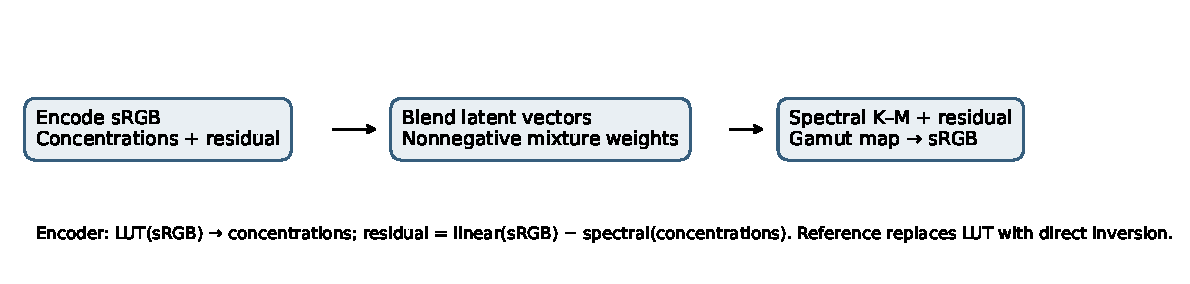
\includegraphics[width=0.94\textwidth,height=0.76\textheight,keepaspectratio]{figures/pipeline.pdf}
\caption{Pipeline. RGB inversion supplies a simplex recipe; its
reconstruction residual is carried alongside the recipe during mixing.}
\end{figure*}

\hypertarget{independently-constructed-pigment-basis}{%
\subsection{4.1 Independently constructed pigment
basis}\label{independently-constructed-pigment-basis}}

We choose eight roles: white, cyan, magenta, yellow, red, green, blue
and black. These are synthetic pigment roles, not measurements of
specific chemical compositions. Define a logistic spectral transition

\[H_e(\lambda)=\left[1+\exp(-(\lambda-e)/w)\right]^{-1},\qquad w=22\ \mathrm{nm}.\]

With edges in nanometers, define shapes \(B=1-H_{510}\), \(Y=H_{530}\),
\(R=H_{600}\), \(C=1-R\), \(G=YC\), and \(M=1-G\). The basis
reflectances are

\[R_i=0.025+0.915b_i,\qquad b_i\in(1,C,M,Y,R,G,B,0).\]

The scattering strengths, in that order, are \((8,1,1,1,1,1,1,0.5)\).
Absorption follows from \(K_i=S_i(1-R_i)^2/(2R_i)\). Positive
reflectance bounds avoid singular absorption and guarantee finite
optical calculations throughout the simplex. These constants are design
priors, not fitted commercial-pigment coefficients. The repository
retains the edge sweep that motivated the selected blue/yellow overlap;
the remaining initial values are explicitly labeled heuristic.

A larger basis offers more possible recipes and introduces ambiguity. It
does not guarantee more realistic behavior. We retain a deterministic
recipe prior and assess smaller subsets rather than assuming that the
eight-component basis is optimal. No source measurement dataset is
silently substituted for the analytic basis.

\begin{figure*}[t]
\centering
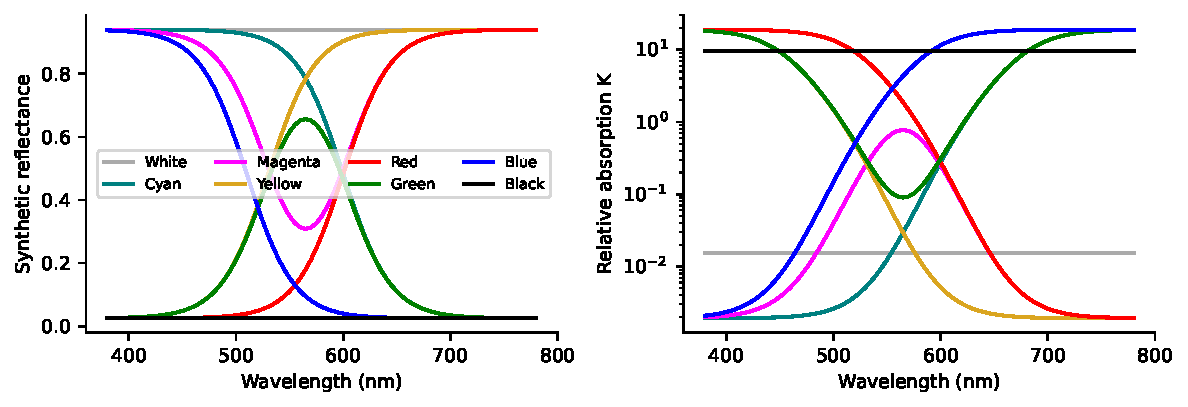
\includegraphics[width=0.94\textwidth,height=0.76\textheight,keepaspectratio]{figures/spectra.pdf}
\caption{Original synthetic reflectance and derived absorption spectra.
White and black are spectrally neutral; their relative scattering
differs.}
\end{figure*}

\hypertarget{constrained-rgb-inversion}{%
\subsection{4.2 Constrained RGB
inversion}\label{constrained-rgb-inversion}}

Let \(F(c)\) be the spectral decoder returning unbounded linear RGB, and
let \(L\) denote conversion from linear RGB to OKLab. For input \(u\)
and decoded \(x\), we approximately minimize

\[J(c;u)=\|L(F(c))-L(x)\|_2^2+\eta\|c-p(u)\|_2^2,\]

subject to the simplex constraints, with \(\eta=0.0002\). The prior
\(p\) is a piecewise-linear cube decomposition in encoded RGB. White
receives the minimum channel and black receives one minus the maximum.
The remaining mass is split between one secondary and one primary
according to sorted channel differences. For example, when
\(r\leq g\leq b\), cyan receives \(g-r\) and blue receives \(b-g\). The
other channel orders are symmetric. The prior is continuous, but its
derivative changes at channel-order boundaries.

The reference solver uses projected Gauss--Newton steps, analytic
derivatives, pivoted dense solves, and backtracking. Differentiation
gives

\[\frac{\partial R}{\partial q}=-\frac{R}{\sqrt{q(q+2)}},\qquad
\frac{\partial q}{\partial c_i}=\frac{K_i-qS_i}{S}.\]

The OKLab chain rule completes the Jacobian. The normal matrix includes
the objective regularizer and a numerical damping term \(10^{-5}\). We
project candidate recipes onto the simplex and accept only objective
decreases exceeding \(10^{-13}\). A projected-gradient fallback is
essential: projection of an unconstrained Newton direction need not
yield descent on a constrained face. The failure of the initial
Newton-only variant was observed in the canonical tests and retained in
the decision log.

There are at most 80 outer iterations, 16 Newton backtracking trials,
and 24 gradient fallback trials. The fallback starts at step size 8 and
halves it. This is a reproducible local algorithm, not a proof of the
globally best concentration vector. The weak prior makes the
underdetermined problem better specified without eliminating local
minima. Independent Python SLSQP calculations are used for exploratory
comparisons and ablations; they are not assumed to yield identical
recipes.

\hypertarget{linear-light-residual-and-mixture-law}{%
\subsection{4.3 Linear-light residual and mixture
law}\label{linear-light-residual-and-mixture-law}}

The encoded latent is \(z=(c,e)\), where \(e=x-F(c)\). For normalized
nonnegative weights \(\alpha_i\), the mixture is

\[\bar c=\sum_i\alpha_ic_i,\quad \bar e=\sum_i\alpha_ie_i,
\quad \bar x=F(\bar c)+\bar e.\]

This construction gives exact reconstruction in real arithmetic because
\(F(c)+[x-F(c)]=x\). The residual may contain negative components and is
not an absorption or scattering coefficient. It supplies a display-space
correction where the physical palette is insufficient. All experiments
therefore distinguish corrected reconstruction, raw palette
approximation and intermediate mixture behavior.

The fast path recomputes the residual after table interpolation using
the actual fast decoder. Interpolating residuals stored only at the
table nodes would not provide the same identity between nodes. For fixed
source latents, concentrations and residuals are affine in the mixture
parameter. The nonlinear K--M decoder produces the resulting curved
color trajectory.

\hypertarget{display-gamut-treatment}{%
\subsection{4.4 Display gamut treatment}\label{display-gamut-treatment}}

The physical decoder and residual can produce out-of-range linear RGB.
We retain raw output for diagnostics and map only for display. For a raw
vector \(x\), set
\(y=\mathrm{clamp}(0.2126x_R+0.7152x_G+0.0722x_B,0,1)\) and
\(d=x-y\mathbf1\). Choose the largest \(a\in[0,1]\) such that
\(y\mathbf1+ad\) lies in the RGB cube. Each positive component of \(d\)
bounds \(a\) by \((1-y)/d_j\); each negative component bounds it by
\(-y/d_j\).

This neutral-axis compression is identity inside the gamut and
continuous at its boundary. It preserves linear luminance when that
luminance is in range. It does not preserve perceptual hue in general.
Beyond the available luminance range the output collapses to black or
white. We count mapping incidence rather than hiding it as an
implementation detail. This simple mapping remains a quality limitation
of the current design.

\hypertarget{reference-and-fast-implementations}{%
\section{5. Reference and fast
implementations}\label{reference-and-fast-implementations}}

\hypertarget{reference-path}{%
\subsection{5.1 Reference path}\label{reference-path}}

The reference samples 380--780 nm inclusive every 5 nm, using 81 f64
values. Trapezoidal integration weights combine D65, observer functions
and the XYZ-to-RGB matrix. A small diagonal normalization maps a perfect
diffuser to exactly \((1,1,1)\), removing the truncated-tabulation white
bias. This is a deliberate approximation to unmodified standard
integration. A 1 nm comparison is included to assess wavelength sampling
for the smooth spectra used here.

The bundled observer and illuminant subset is obtained through Colour
0.4.6. Observer samples are at 1 nm; the package's 5 nm D65 samples are
linearly interpolated to 1 nm before subsampling. We do not claim byte
identity with the current official CIE CSV files. The exact subset
checksum, source attribution and transformation are recorded. Standard
colorimetric data and derived assets retain their documented CC BY-SA
terms, separately from the MIT OR Apache-2.0 source code.

The reference is ground truth only for approximation comparisons within
this synthetic model. It is not ground truth for a real paint sample.
That distinction applies both to error statistics and to the word
reference in the public API.

\hypertarget{lookup-table-encoder}{%
\subsection{5.2 Lookup-table encoder}\label{lookup-table-encoder}}

We sample the encoded RGB cube uniformly at resolutions 17³, 33³ and
65³. Every node stores eight f32 concentrations generated by the same
reference optimizer. No neighbor warm start is used, so generation order
cannot affect a node's initialization. The table is regenerated by a
separate executable; no unexplained binary coefficients are required.

At a query, sort the three fractional cell coordinates as
\(f_a\geq f_b\geq f_c\). The tetrahedron's four interpolation weights
are \((1-f_a,f_a-f_b,f_b-f_c,f_c)\). They are nonnegative and sum to
one, preserving the recipe simplex. Shared-face agreement gives a
continuous encoder even if the optimized node recipes vary sharply. It
does not make the encoder differentiable, remove steep local changes, or
make an ambiguous inverse unique. A trilinear eight-vertex encoder is
included for comparison.

Having eight output pigments does not prevent a 3D encoder table because
its domain is RGB. It does prevent a general unrestricted concentration
decoder from being represented by an ordinary 3D table. We therefore
evaluate the decoder spectrally instead of claiming that all latent
dimensions can be indexed by the RGB table.

\hypertarget{reduced-spectral-decoder-and-runtime-api}{%
\subsection{5.3 Reduced spectral decoder and runtime
API}\label{reduced-spectral-decoder-and-runtime-api}}

The fast decoder uses 21 samples at 20 nm in f32, with fixed-size stack
arrays and precombined colorimetric weights. It evaluates the same
positive K--M formula and palette. We measure sampling and
floating-point effects separately where possible. No hand-written SIMD,
fitted polynomial decoder, neural network, Rayon or GPU kernel is
implemented. The compiler's ordinary optimizations are not labeled a
custom vectorized implementation.

The public API accepts checked sRGB colors, pair interpolation and
arbitrary nonnegative weighted mixtures. Invalid weights return an
error. A convenience pair API clamps \(t\) and maps NaN to the first
endpoint; a checked alternative rejects invalid \(t\). Pair endpoints
are returned exactly. The latent structures keep their internal
concentrations private and provide read-only accessors. Raw decode is
available for scientific inspection.

A complete RGB mixture decodes three spectra: one for each input's
residual and one for the mixed recipe. Cached latent mixing decodes only
the result. Applications should retain a mixer object and cache paint
latents where possible. The embedded default table is parsed once and
shared immutably. No per-mixture heap allocation, external crate, unsafe
code, file operation or network access is required in the runtime.

\hypertarget{experimental-methodology}{%
\section{6. Experimental methodology}\label{experimental-methodology}}

The evaluation uses 10000 uniformly sampled encoded-RGB colors and 10000
independent random color pairs with uniformly sampled \(t\). Rust uses
an explicitly implemented xorshift64 sequence seeded with 20260929;
exploratory Python ablations use NumPy's documented generator with the
same integer seed, which does not imply identical sequences. Sample CSV
files accompany the release, allowing metrics to be recalculated without
regenerating the random streams.

Reconstruction is assessed in CIEDE2000 (Sharma, Wu, and Dalal 2005),
\(100\|\Delta\mathrm{OKLab}\|\), and channel error. Colour 0.4.6
provides the independent CIEDE2000 implementation. We report mean,
median, 95th percentile, 99th percentile and maximum. We evaluate the
uncorrected palette after the same display gamut map rather than
measuring only the algebraically restored endpoints. Raw linear channels
are also retained.

Mixing comparisons include encoded-sRGB interpolation, linear-RGB
interpolation, OKLab interpolation, the fast hybrid, the reference
hybrid and the fast decoder without residuals. Twelve canonical pairs
cover primaries, secondaries, complements, tints, neutrals and an
extreme yellow--blue case. Each trajectory uses 1001 samples. These
examples were specified before the final Rust experiment. They are
useful diagnostics, not a representative distribution of artists' paint
choices. There is no blinded perceptual study or measured physical
target.

The spectral sampling ablation fixes the recorded reference
concentrations and reevaluates them at 1, 5, 10, 20 and 40 nm. This
isolates the forward approximation from inverse selection. The palette
ablation uses 128 common colors and the same independent SLSQP procedure
for CMYW, CMYWK, eight pigments, removal of white, and equal
white/chromatic scattering. It measures each subset's uncorrected
approximation; residual-corrected reconstruction would hide the effect
under investigation.

Runtime tests use one native thread, varying colors and \(t\) from a
seeded workload, and compiler barriers to prevent dead-code removal.
Seven repetitions are recorded. Most modes run 100000 operations per
repetition; direct reference inversion is limited to 1000 because of its
cost. Timings include the public color-output conversion where that
method returns RGB. Lookup-only timings are labeled separately. Table
parsing is measured separately from steady-state mixing, and offline
generation wall time is recorded. There is no direct benchmarking of
Mixbox or other proprietary software.

The host reports AMD EPYC 9V74 80-Core Processor. The build uses Rust
1.75.0, release optimization, one code-generation unit, no LTO and no
target-cpu=native flag. The full environment record is included. Host
scheduling and frequency are uncontrolled; these are local
microbenchmarks, not universal performance guarantees. No browser/WASM
throughput is inferred from them.

\hypertarget{results}{%
\section{7. Results}\label{results}}

\hypertarget{endpoint-consistency-and-palette-limitations}{%
\subsection{7.1 Endpoint consistency and palette
limitations}\label{endpoint-consistency-and-palette-limitations}}

\begin{table*}[t]
\caption{Source reconstruction (CIEDE2000).}
\centering\small
\begin{tabular}{@{}llllll@{}}
\toprule\noalign{}
Model & Mean & Median & P95 & P99 & Max \\
\midrule\noalign{}

\bottomrule\noalign{}

Reference + residual & 0 & 0 & 0 & 0 & 0 \\
Fast + residual & 1.19e-07 & 0 & 6.86e-07 & 1.17e-06 & 2.38e-06 \\
Reference palette only & 11.7 & 9.58 & 28.4 & 34.6 & 42 \\
Fast palette only & 11.8 & 9.65 & 28.4 & 35 & 42.3 \\
\end{tabular}
\end{table*}

Corrected reconstruction is near floating-point precision, as expected.
The uncorrected palette has substantially larger error. Its worst
regions are exposed in the heatmap and top-error CSV rather than
excluded as unusual inputs. Saturated display colors are particularly
difficult because broad positive-reflectance pigments do not span the
display cube. This model deliberately trades unrestricted RGB gamut for
an explicit material prior.

The forward implementation cross-check, evaluating the recorded Rust
recipes in independent Python f64 code, has maximum linear-channel
difference 1.31e-13. This validates agreement of equations, coefficients
and integration for identical recipes. It does not validate the recipes
against physical measurements. The 20 nm f32 check, including
concentration rounding, has maximum linear-channel discrepancy 3.2e-07
against f64. The wavelength study further separates arithmetic accuracy
from modeling accuracy.

\begin{figure*}[t]
\centering
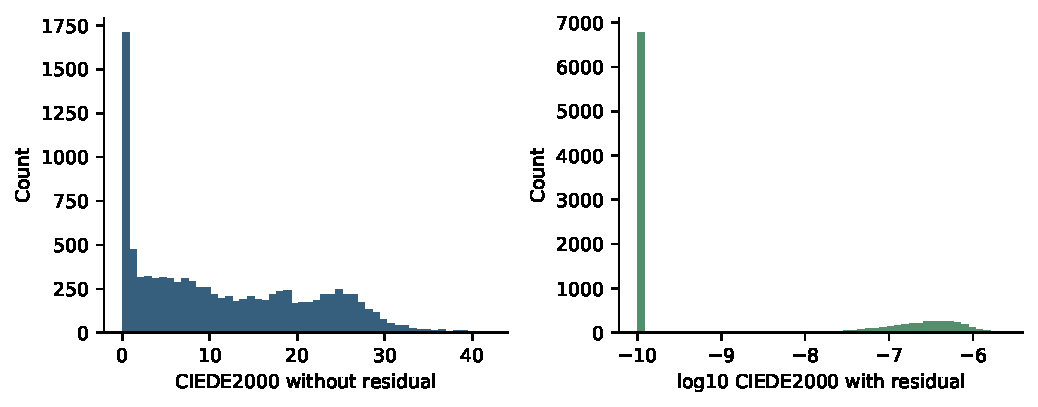
\includegraphics[width=0.94\textwidth,height=0.76\textheight,keepaspectratio]{figures/error_histogram.pdf}
\caption{Reconstruction error distributions. The left plot measures the
palette alone; the right shows the tiny numerical error after residual
correction on a logarithmic scale.}
\end{figure*}

\begin{figure*}[t]
\centering
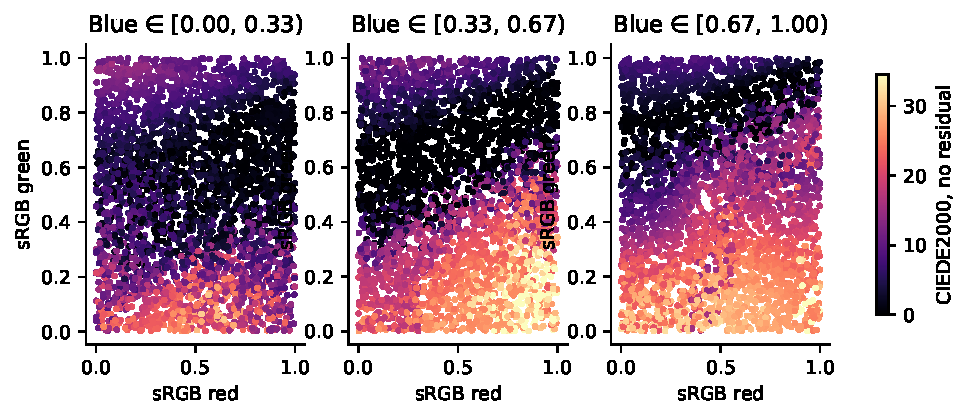
\includegraphics[width=0.94\textwidth,height=0.76\textheight,keepaspectratio]{figures/reconstruction_heatmap.pdf}
\caption{Systematic view of uncorrected palette error over random RGB
samples, divided into blue-channel slices. No sample is removed for
having high error.}
\end{figure*}

\hypertarget{canonical-mixtures-and-gamut-mapping}{%
\subsection{7.2 Canonical mixtures and gamut
mapping}\label{canonical-mixtures-and-gamut-mapping}}

\begin{table*}[t]
\caption{Canonical fast-model midpoint colors.}
\centering\small
\begin{tabular}{@{}ll@{}}
\toprule\noalign{}
Pair & Fast midpoint (sRGB8) \\
\midrule\noalign{}

\bottomrule\noalign{}

black + white & (141, 141, 141) \\
blue + orange & (103, 87, 91) \\
blue + white & (107, 188, 255) \\
cyan + magenta & (148, 101, 130) \\
extreme + yellow + blue & (60, 174, 124) \\
magenta + yellow & (237, 120, 116) \\
red + blue & (88, 0, 71) \\
red + green & (137, 100, 39) \\
red + white & (255, 166, 124) \\
red + yellow & (242, 118, 14) \\
yellow + blue & (49, 144, 112) \\
yellow + purple & (162, 130, 134) \\
\end{tabular}
\end{table*}

The selected yellow--blue trial bends into green; red--blue gives a dark
purple rather than an additive average. Complementary examples reduce
chroma, and adding white changes both the amount and trajectory of
lightening because scattering is mixed separately from absorption. The
cyan--magenta midpoint is muted rather than a clean saturated blue, and
the red--white tint shifts markedly toward peach. These are visible
compromises of this chosen basis and residual convention. Nevertheless,
the examples do not establish material fidelity. A paint identified only
as red or blue could have a different spectral tail and very different
mixing behavior.

8.42\% of the random fast mixtures require display gamut mapping. The
raw linear output range across those trials is {[}-0.209, 1.061{]}. This
is evidence that residual correction and the physical basis sometimes
disagree substantially. The mapper maintains bounded output and
continuity, but may compress chroma and distort hue. Those effects
appear in the trajectory plots and must be addressed before claiming a
high-fidelity professional paint simulation.

\begin{figure*}[t]
\centering
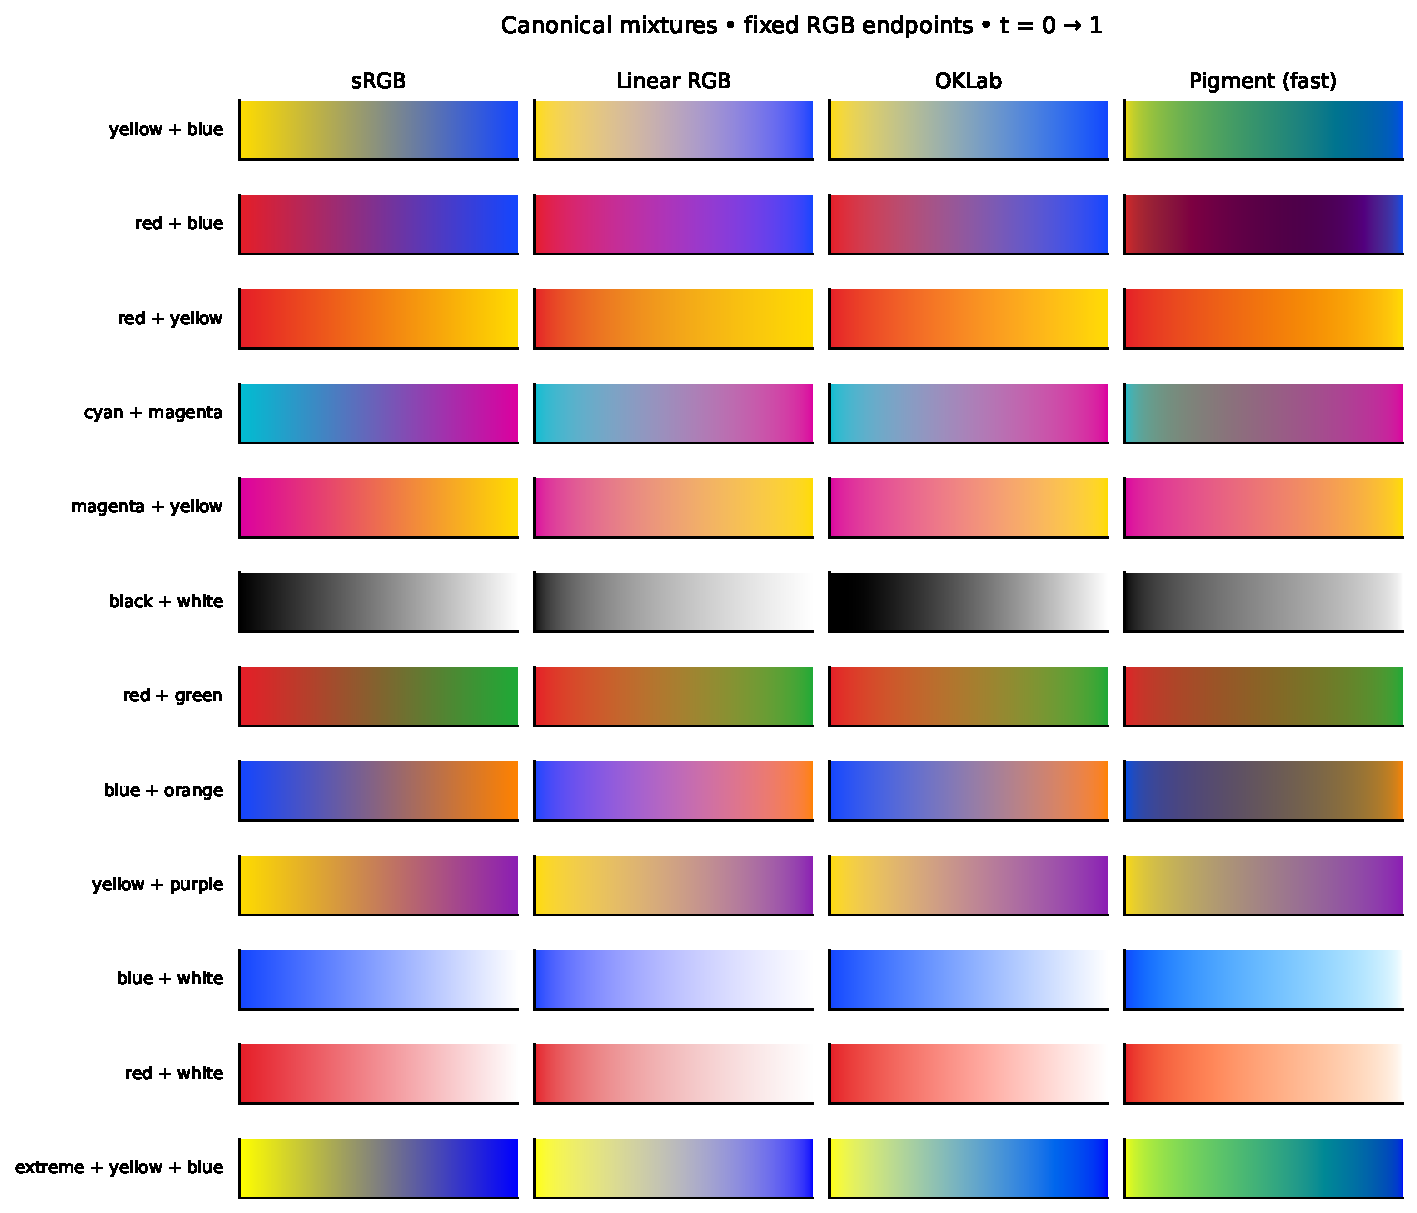
\includegraphics[width=0.94\textwidth,height=0.76\textheight,keepaspectratio]{figures/comparisons.pdf}
\caption{Canonical gradients, with identical endpoints and mixture
parameters across methods. All rows, including difficult complement and
tint cases, are shown.}
\end{figure*}

\begin{figure*}[t]
\centering
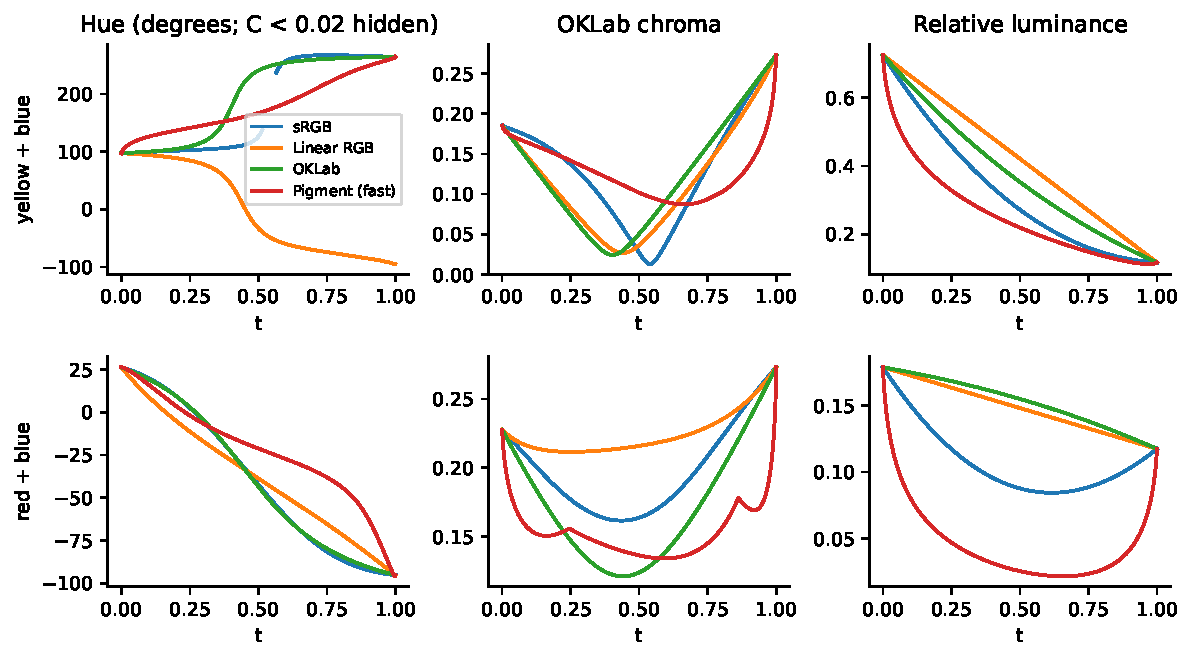
\includegraphics[width=0.94\textwidth,height=0.76\textheight,keepaspectratio]{figures/trajectories.pdf}
\caption{Hue, chroma and luminance trajectories. Hue is hidden below
OKLab chroma 0.02 because its angle is unstable near neutral. Curvature
and nonmonotonic luminance can be legitimate outcomes, but are not
independently validated paint behavior.}
\end{figure*}

\hypertarget{table-approximation-and-spectral-sampling}{%
\subsection{7.3 Table approximation and spectral
sampling}\label{table-approximation-and-spectral-sampling}}

\begin{table*}[t]
\caption{Mixture error relative to direct reference (CIEDE2000).}
\centering\small
\begin{tabular}{@{}llllll@{}}
\toprule\noalign{}
Encoder & Mean & Median & P95 & P99 & Max \\
\midrule\noalign{}

\bottomrule\noalign{}

n17 & 0.706 & 0.184 & 2.55 & 10.9 & 43.8 \\
n33 & 0.409 & 0.0918 & 1.19 & 6.48 & 40.1 \\
n65 & 0.265 & 0.0631 & 0.774 & 4.19 & 36.7 \\
tri33 & 0.438 & 0.0994 & 1.38 & 6.93 & 40.5 \\
\end{tabular}
\end{table*}

These errors compare full displayed mixtures against the direct
reference model, rather than comparing only table-node reconstructions.
The default 33³ table is a memory/approximation compromise. Each node
occupies 32 bytes, giving 157,216, 1,149,984 and 8,788,000 bytes of
concentration payload at the three resolutions; the binary header adds
eight bytes. The maximum 33³ discrepancy of 40.1 CIEDE2000 is a material
failure of uniform approximation. Low average error does not make the
table a reliable substitute in every RGB region. The worst examples
involve large changes in selected recipe and residual, exposed in the
supplementary worst-case figure. Increasing the table resolution changes
both local interpolation and how closely the fast path follows the
reference inverse's recipe choices. A local inverse is not necessarily a
globally smooth target, so monotonic quality improvements should not be
assumed.

The 20 nm forward model, evaluated in f64 at fixed recipes, has mean
CIEDE2000 0.0826 and 95th-percentile 0.149 relative to 5 nm. This
isolates sampling error from the LUT's inverse approximation. Since the
analytic spectra are smooth and broad, the coarse sampling is more
successful than it would necessarily be for narrow-band or measured
interference pigments. The 1 nm comparison is a numerical check of this
restricted basis, not a claim that all paint spectra can be represented
at 20 nm.

\begin{figure*}[t]
\centering
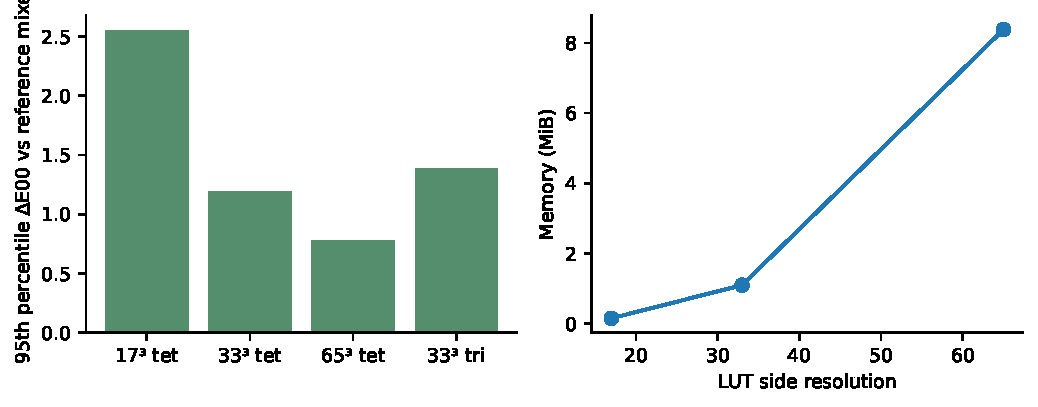
\includegraphics[width=0.94\textwidth,height=0.76\textheight,keepaspectratio]{figures/lut_resolution.pdf}
\caption{LUT approximation versus reference mixtures, and table memory.
The trilinear variant uses the same 33³ node data.}
\end{figure*}

\hypertarget{smoothness}{%
\subsection{7.4 Smoothness}\label{smoothness}}

All recorded canonical displayed samples are finite. The largest
adjacent-step difference among fast canonical trajectories is 7.75
\ensuremath{\Delta}EOK100 at the tested spacing. A separate 200-pair, 1,001-step random
test has largest adjacent step 6.42. The random maximum is perceptually
substantial over a small parameter change and fails a stronger
requirement of uniformly gentle visual transitions. These sampled bounds
do not prove perceptual smoothness for all inputs. The mathematical
argument is more specific: convex concentration interpolation stays in a
positive optical domain; K--M decoding and the residual are continuous;
the gamut map is continuous. Derivative kinks can still arise from gamut
boundaries, table faces or channel-order changes.

The tests separately probe source reconstruction, exact pair endpoints,
symmetry, nonnegative normalized weights, nonfinite input handling,
malformed tables, and crossings of LUT cell boundaries. Eight-bit output
can still band even when the floating-point curve is continuous.
Retaining floating-point canvas data and applying an appropriate
display/dithering strategy remains the host application's
responsibility.

\hypertarget{runtime-performance}{%
\subsection{7.5 Runtime performance}\label{runtime-performance}}

\begin{table*}[t]
\caption{Single-thread native timing; lookup is not a full mix.}
\centering\small
\begin{tabular}{@{}lll@{}}
\toprule\noalign{}
Operation & Median ns & Million/s \\
\midrule\noalign{}

\bottomrule\noalign{}

sRGB & 19.2 & 52 \\
linear RGB & 160 & 6.27 \\
OKLab & 245 & 4.07 \\
reference RGB & 2.39e+06 & 0.000418 \\
fast RGB & 602 & 1.66 \\
fast cached latent & 226 & 4.42 \\
tetrahedral lookup & 34.8 & 28.7 \\
reference cached latent & 835 & 1.2 \\
trilinear lookup & 34 & 29.4 \\
\end{tabular}
\end{table*}

The median full fast RGB operation costs 602 ns and the cached latent
operation costs 226 ns on this host. The cost difference follows the
number of spectral evaluations and input transfer functions, not a
change in the mixture law. Lookup alone is faster but is not the
complete mixing operation and must not be advertised as such. The
default table parsing median is 0.267 ms. Offline generation durations
are retained in the performance dataset; they are excluded from
steady-state timing.

\begin{figure*}[t]
\centering
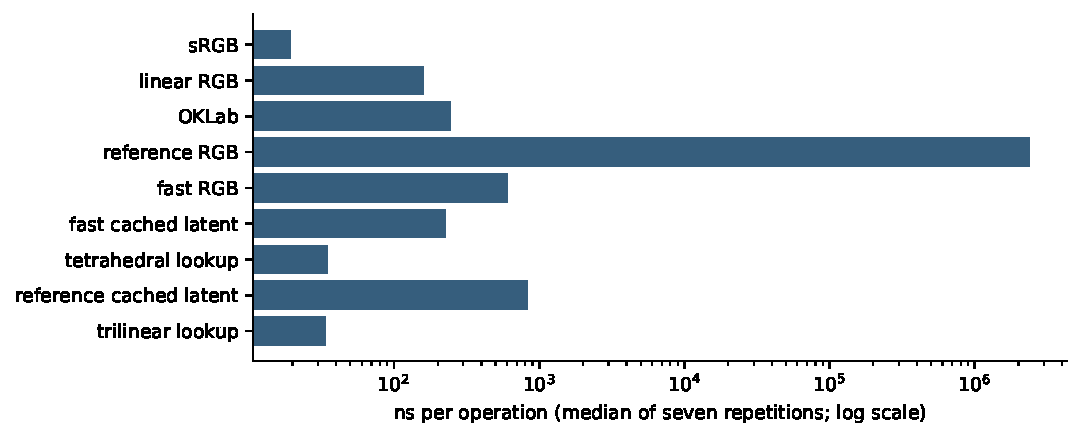
\includegraphics[width=0.94\textwidth,height=0.76\textheight,keepaspectratio]{figures/performance.pdf}
\caption{Single-thread native operation costs, with logarithmic
horizontal scale. Direct inversion, full RGB mixing, cached latent
mixing, and lookup alone are different workloads.}
\end{figure*}

\hypertarget{ablations-and-negative-findings}{%
\section{8. Ablations and negative
findings}\label{ablations-and-negative-findings}}

\begin{table*}[t]
\caption{Palette and scattering ablations, without residual (CIEDE2000).}
\centering\small
\begin{tabular}{@{}lllll@{}}
\toprule\noalign{}
Basis / S variant & Mean & Median & P95 & Max \\
\midrule\noalign{}

\bottomrule\noalign{}

CMYW & 23.6 & 23.2 & 49.6 & 64.3 \\
CMYWK & 15.7 & 15.1 & 28.6 & 30.2 \\
eight & 11.7 & 7.06 & 29.7 & 38.1 \\
no white & 12.1 & 7.68 & 30 & 38.1 \\
equal scattering & 11.7 & 7.06 & 29.7 & 38.1 \\
\end{tabular}
\end{table*}

The subset experiment measures representation power under a common
optimizer and source sample set. Removing components can force a larger
residual, but a larger basis can also create additional recipe choices.
We therefore interpret improvements in raw reconstruction as increased
colorimetric flexibility, not automatic improvement in mixture realism.
Removing white is particularly relevant to tints, while equalizing
scattering changes mixing strength without necessarily changing the
isolated pigment colors.

The first full-spectrum trial used a bounded,
first-difference-regularized reflectance reconstruction, followed by
constant-scattering K--M. Its black--white midpoint was approximately
(7,7,7) in 8-bit sRGB. The reconstructed black's large K/S dominated the
mixture. This is a concrete example of why colorimetric reconstruction
alone is insufficient. The selected palette represents black with finite
absorption, an explicit relative scattering, and a residual for the
remaining endpoint mismatch.

The initial palette put the blue edge at 500 nm and the yellow edge at
490 nm. Its corrected yellow--blue midpoint was (19,128,145), too cyan
for the target example. Moving both edges to 530 nm improved green
overlap but caused the red--blue trial to collapse to black after
residual correction and mapping. We retained a 510 nm blue edge and 530
nm yellow edge as a compromise. This is limited tuning on diagnostic
examples and is openly identified as such; the subsequent random trials
assess behavior outside those examples.

The first Rust inversion used only projected unconstrained Gauss--Newton
steps. A canonical hue test failed because projection could destroy
descent on an active constraint face. Adding projected-gradient fallback
corrected that numerical failure. We did not weaken the test to accept
the faulty result. The independent Python optimizer helped identify that
the problem was inversion, rather than the K--M forward equations.

\begin{figure*}[t]
\centering
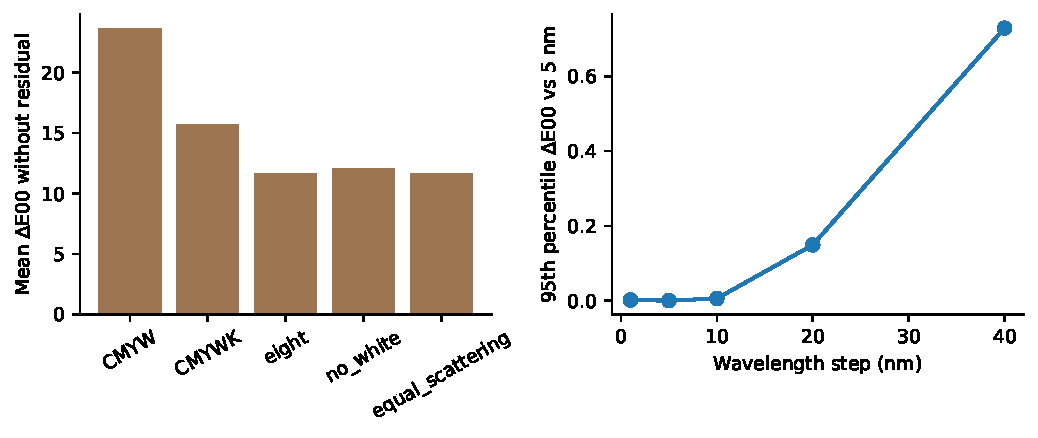
\includegraphics[width=0.94\textwidth,height=0.76\textheight,keepaspectratio]{figures/ablations.pdf}
\caption{Palette/scattering ablations and fixed-recipe spectral-sampling
error. The left experiment uses the independent SLSQP solver on a common
128-color set.}
\end{figure*}

No negative conclusions are claimed for neural encoders, polynomial
decoders, SIMD, GPU implementations or measured pigment fitting: these
were reviewed or proposed, but not experimentally implemented.
Distinguishing a rejected hypothesis from an untested option is
necessary for a reproducible research record.

\begin{figure*}[t]
\centering
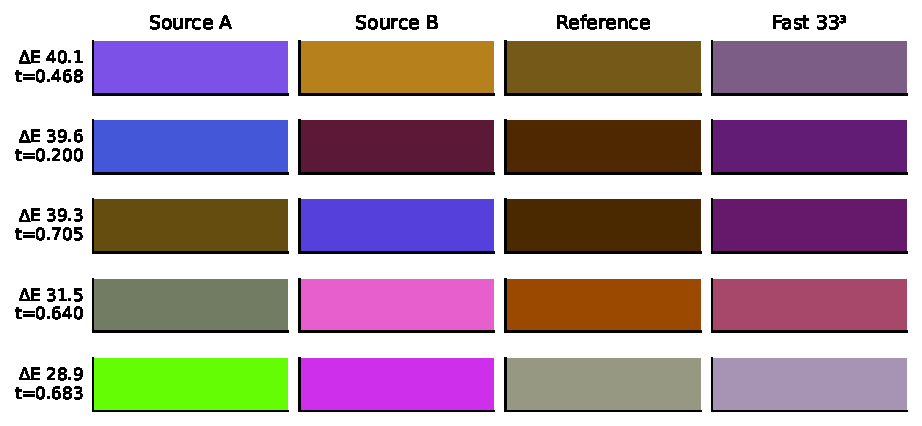
\includegraphics[width=0.94\textwidth,height=0.76\textheight,keepaspectratio]{figures/worst_cases.pdf}
\caption{The five largest default-LUT discrepancies in the random-pair
experiment. Both outputs are model predictions; neither is a
measured-paint target. The large disagreements expose a weakness that
mean error alone hides.}
\end{figure*}

\hypertarget{discussion}{%
\section{9. Discussion}\label{discussion}}

The most favorable reconstruction statistic is also the easiest to
misinterpret. A residual makes arbitrary RGB reconstruction nearly exact
by construction. This is useful engineering: pasted artwork and
arbitrary color-picker values can be accepted without an endpoint color
shift. It does not show that a small physical palette spans RGB, that
the inferred spectrum is correct, or that intermediate colors match real
mixtures. Reporting the palette-only error and mapping incidence is
therefore essential.

The eight-component palette retains more flexible recipes than a
four-component palette, but RGB provides fewer constraints than the
recipe has degrees of freedom. Regularization chooses a convention. The
LUT then approximates that convention. There is no reason to expect two
independent solvers with different priors to produce the same
intermediate color even if both reconstruct the endpoints. This is a
design space for artistic evaluation, not an error that can be removed
simply by increasing numerical precision.

Spectral work remains inexpensive enough to be useful after the inverse
is precomputed. The current CPU implementation spends a fixed amount of
work on a small number of smooth bands. A polynomial or neural decoder
could reduce that work further, but would need to preserve positivity,
endpoint correction, and the observed curve quality. The measured
cached-latent path establishes a concrete baseline against which such
complexity should be justified.

The representation also clarifies a canvas-design decision. An RGB-only
canvas repeatedly discards the inferred recipe after displaying each
result. Re-encoding can produce a new recipe. Consequently a sequence of
RGB pair operations is not generally associative, even though normalized
linear combinations of retained latents are. An application that needs
persistent material history should store latent recipes and paint
amounts, or spectral state, alongside its display buffer. A drop-in RGB
mixer cannot preserve information the host discards.

Adding white is especially revealing. Raising the white scattering
coefficient produces stronger tinting without changing the isolated
white reflectance. This behavior is consistent with the model's
separation of absorption and scattering, but the selected coefficient is
not calibrated to titanium white. A future dataset should contain either
separate optical coefficients or enough thickness/backing/mixture
observations to estimate them. A collection of opaque RGB swatches is
not sufficient for this calibration.

\hypertarget{limitations}{%
\section{10. Limitations}\label{limitations}}

The principal limitation is the lack of measured pigment-mixture
validation and artist evaluation. The spectra, scattering strengths and
selected edge positions are synthetic priors. Some display colors
require large residuals; gamut mapping is frequent enough to matter and
can alter perceptual hue. The local inverse has no global-optimality
guarantee, and LUT continuity does not guarantee gentle gradients with
respect to every possible input perturbation.

The model assumes a homogeneous, opaque, diffuse layer under one
illuminant and observer. It does not represent finite paint thickness,
translucent glazing, gloss, fluorescence, metallic or interference
pigments, particle-size-dependent scattering, granulation, or spatial
pigment segregation. It does not predict wetness, drying, canvas
absorption or brush transport. The RGB residual is not a spectrum, so
relighting the corrected color under a different illuminant is not
physically defined by the current representation.

Numerical evaluation is restricted to the declared synthetic basis and
sample distributions. Random RGB samples are not a distribution of
real-world paints. The fine-sampling comparison does not cover sharply
structured measured spectra. Performance is native, scalar-source,
single-host evidence; the WASM CI target is a portability check, not a
browser benchmark. The release is not presented as externally reviewed,
deployed in a production painting program or peer-reviewed.

\hypertarget{future-work}{%
\section{11. Future work}\label{future-work}}

The highest-value next experiment is a permissively redistributable
dataset of measured mixtures, including tints and multiple application
thicknesses or backings. This would support fitting K and S separately,
comparing spectral errors as well as colorimetric errors, and testing
whether the synthetic palette's successful examples survive
material-specific calibration. A blinded artist study could then
evaluate useful behavior beyond named-color expectations.

The inverse could incorporate neighborhood regularization across the
LUT, a constrained surrogate optimizer, or a learned predictor with a
reproducible training set. Such methods should be assessed on recipe
stability and intermediate mixtures, not just endpoint RGB. A larger
palette should be justified by measured gains and manageable ambiguity.
Alternative gamut mapping should be evaluated on the currently recorded
out-of-range cases rather than only visually favorable gradients.

For performance, batching and SIMD are straightforward candidates
because wavelengths and independent pixels admit parallel work. GPU and
WASM implementations require their own precision and timing studies. A
fitted decoder may reduce runtime spectral integration, but should
retain a reference spectral mode for validation. Finite-layer K--M,
backing interactions and a physically specified binder would be required
for glazing. Wet-on-wet and oil- or watercolor-specific behavior would
additionally require transport and material-state models.

\hypertarget{conclusion}{%
\section{12. Conclusion}\label{conclusion}}

This study implements an independent, reproducible RGB pigment-mixing
research library using public K--M equations and a published
concentration-plus-residual representation. The selected synthetic basis
produces the intended green and purple canonical mixtures and supports
arbitrary sRGB endpoints with near-floating-point reconstruction error.
That endpoint result is algebraic, while the uncorrected palette error
of 11.7 mean CIEDE2000 exposes the basis's limitations.

The default fast model reaches 1.66 million complete RGB mixtures per
second, and 4.42 million cached-latent mixtures per second on the
measured host. Its random-mixture mean discrepancy from the reference is
0.409 CIEDE2000. The project therefore establishes a usable
implementation and performance baseline, together with clear unresolved
quality risks: synthetic material priors, large residuals for some
inputs, inverse ambiguity and gamut mapping. It is suitable for
integration experiments and further validation. A claim of calibrated or
professional-grade paint fidelity would require evidence this study does
not yet provide.

\hypertarget{reproducibility-and-authorship-note}{%
\section{Reproducibility and authorship
note}\label{reproducibility-and-authorship-note}}

\texttt{python3\ tools/reproduce.py} regenerates model arrays, all three
encoder tables, tests, raw experiment outputs, metrics, figures and this
manuscript's result tables. The bundled data permit offline runtime
builds. Python dependencies and model settings are pinned or recorded;
\texttt{results/environment.json} and the source/data manifest identify
the reported configuration. The accompanying Markdown, TeX, bibliography
and CSV files are the primary research record. This is an AI-assisted
implementation and manuscript prepared for the commissioning user, with
measurements produced by executable repository experiments. It has not
undergone external peer review.

\hypertarget{references}{%
\section*{References}\label{references}}
\addcontentsline{toc}{section}{References}

\hypertarget{refs}{}
\begin{CSLReferences}{1}{0}
\leavevmode\vadjust pre{\hypertarget{ref-burns2020}{}}%
Burns, Scott Allen. 2020. {``Numerical Methods for Smoothest Reflectance
Reconstruction.''} \emph{Color Research and Application} 45: 8--21.
\url{https://doi.org/10.1002/col.22437}.

\leavevmode\vadjust pre{\hypertarget{ref-colour}{}}%
Colour Developers. n.d. {``Colour: Colour Science for Python, Version
0.4.6.''} \url{https://github.com/colour-science/colour}.

\leavevmode\vadjust pre{\hypertarget{ref-curtis1997}{}}%
Curtis, Cassidy J., Sean E. Anderson, Joshua E. Seims, Kurt W.
Fleischer, and David H. Salesin. 1997. {``Computer-Generated
Watercolor.''} In \emph{Proceedings of SIGGRAPH}, 421--30.
\url{https://grail.cs.washington.edu/projects/watercolor/}.

\leavevmode\vadjust pre{\hypertarget{ref-gossett2004}{}}%
Gossett, Nathan, and Baoquan Chen. 2004. {``Paint Inspired Color Mixing
and Compositing for Visualization.''} In \emph{IEEE Symposium on
Information Visualization}, 113--18.
\url{https://doi.org/10.1109/INFOVIS.2004.52}.

\leavevmode\vadjust pre{\hypertarget{ref-haase1992}{}}%
Haase, Chet S., and Gary W. Meyer. 1992. {``Modeling Pigmented Materials
for Realistic Image Synthesis.''} \emph{ACM Transactions on Graphics} 11
(4): 305--35. \url{https://doi.org/10.1145/146443.146452}.

\leavevmode\vadjust pre{\hypertarget{ref-hebert2015}{}}%
Hébert, Mathieu, and Roger D. Hersch. 2015. {``Review of Spectral
Reflectance Models for Halftone Prints: Principles, Calibration, and
Prediction Accuracy.''} \emph{Color Research and Application}.
\url{https://doi.org/10.1002/col.21907}.

\leavevmode\vadjust pre{\hypertarget{ref-cied65}{}}%
International Commission on Illumination. 2019a. {``{CIE} Standard
Illuminant {D65}.''} \url{https://doi.org/10.25039/CIE.DS.hjfjmt59}.

\leavevmode\vadjust pre{\hypertarget{ref-cieobserver}{}}%
---------. 2019b. {``Colour-Matching Functions of {CIE} 1931 Standard
Colorimetric Observer.''}
\url{https://doi.org/10.25039/CIE.DS.xvudnb9b}.

\leavevmode\vadjust pre{\hypertarget{ref-jakob2019}{}}%
Jakob, Wenzel, and Johannes Hanika. 2019. {``A Low-Dimensional Function
Space for Efficient Spectral Upsampling.''} \emph{Computer Graphics
Forum} 38 (2). \url{https://doi.org/10.1111/cgf.13626}.

\leavevmode\vadjust pre{\hypertarget{ref-kubelka1948}{}}%
Kubelka, Paul. 1948. {``New Contributions to the Optics of Intensely
Light-Scattering Materials. Part i.''} \emph{Journal of the Optical
Society of America} 38 (5): 448--57.
\url{https://doi.org/10.1364/JOSA.38.000448}.

\leavevmode\vadjust pre{\hypertarget{ref-kubelka1931}{}}%
Kubelka, Paul, and Franz Munk. 1931. {``Ein Beitrag Zur Optik Der
Farbanstriche.''} \emph{Zeitschrift f{ü}r Technische Physik} 12:
593--601.

\leavevmode\vadjust pre{\hypertarget{ref-ottosson2020}{}}%
Ottosson, Björn. 2020. {``A Perceptual Color Space for Image
Processing.''} \url{https://bottosson.github.io/posts/oklab/}.

\leavevmode\vadjust pre{\hypertarget{ref-sharma2005}{}}%
Sharma, Gaurav, Wencheng Wu, and Edul N. Dalal. 2005. {``The {CIEDE2000}
Color-Difference Formula: Implementation Notes, Supplementary Test Data,
and Mathematical Observations.''} \emph{Color Research and Application}
30 (1): 21--30. \url{https://doi.org/10.1002/col.20070}.

\leavevmode\vadjust pre{\hypertarget{ref-smits1999}{}}%
Smits, Brian. 1999. {``An {RGB}-to-Spectrum Conversion for
Reflectances.''} \emph{Journal of Graphics Tools} 4 (4): 11--22.
\url{https://doi.org/10.1080/10867651.1999.10487511}.

\leavevmode\vadjust pre{\hypertarget{ref-sochorova2021}{}}%
Sochorová, Šárka, and Ondřej Jamriška. 2021. {``Practical Pigment Mixing
for Digital Painting.''} \emph{ACM Transactions on Graphics} 40 (6):
234:1--11. \url{https://doi.org/10.1145/3478513.3480549}.

\leavevmode\vadjust pre{\hypertarget{ref-tan2017}{}}%
Tan, Jianchao, Stephen DiVerdi, Jingwan Lu, and Yotam Gingold. 2017.
{``Pigmento: Pigment-Based Image Analysis and Editing.''}
\url{https://arxiv.org/abs/1707.08323}.

\leavevmode\vadjust pre{\hypertarget{ref-csscolor}{}}%
World Wide Web Consortium. n.d. {``{CSS} Color Module Level 4.''}
\url{https://www.w3.org/TR/css-color-4/}.

\end{CSLReferences}

\end{document}
